\documentclass[11pt]{article}

\usepackage{fullpage}
\usepackage{graphicx}
\usepackage{amsmath}
\usepackage{amssymb}
\usepackage{amsthm}
\usepackage{fancyvrb}

\parindent0in
\pagestyle{plain}
\thispagestyle{plain}

\newcommand{\myname}{Mehshan Mustafa}
\newcommand{\dated}{\today}

\newenvironment{theorem}[2][Theorem]{\begin{trivlist}
\item[\hskip \labelsep {\bfseries #1}\hskip \labelsep {\bfseries #2.}]}{\end{trivlist}}
\newenvironment{lemma}[2][Lemma]{\begin{trivlist}
\item[\hskip \labelsep {\bfseries #1}\hskip \labelsep {\bfseries #2.}]}{\end{trivlist}}
\newenvironment{exercise}[2][Exercise]{\begin{trivlist}
\item[\hskip \labelsep {\bfseries #1}\hskip \labelsep {\bfseries #2.}]}{\end{trivlist}}
\newenvironment{problem}[2][Problem]{\begin{trivlist}
\item[\hskip \labelsep {\bfseries #1}\hskip \labelsep {\bfseries #2.}]}{\end{trivlist}}
\newenvironment{question}[2][Question]{\begin{trivlist}
\item[\hskip \labelsep {\bfseries #1}\hskip \labelsep {\bfseries #2.}]}{\end{trivlist}}
\newenvironment{corollary}[2][Corollary]{\begin{trivlist}
\item[\hskip \labelsep {\bfseries #1}\hskip \labelsep {\bfseries #2.}]}{\end{trivlist}}
\newenvironment{solution}{\begin{proof}[Solution]}{\end{proof}}
\newenvironment{idea}[2][Proof Idea.]{\textit{#1} #2}

\begin{document}

\textbf{Introduction to the Theory of
Computation}\hfill\textbf{\myname}\\[0.01in]
\textbf{Chapter 1: Reqular Languages}\hfill\textbf{\dated}\\
\smallskip\hrule\bigskip

\begin{problem}{1.32}
Let
\[
\Sigma_{3} = 
\left\{
\begin{bmatrix}
    0 \\
    0 \\
    0
\end{bmatrix} ,
\begin{bmatrix}
    0 \\
    0 \\
    1
\end{bmatrix} ,
\begin{bmatrix}
    0 \\
    1 \\
    0
\end{bmatrix} ,
\, \hdots \, ,
\begin{bmatrix}
    1 \\
    1 \\
    1
\end{bmatrix}
\right\}
\]
\\
$\Sigma_{3}$ contains all size 3 columns of 0s and 1s. A string of symbols in $\Sigma_{3}$ gives three rows of 0s and 1s. Consider each row to be a binary number and let
\[
B = 
\left\{
w \in \Sigma_{3}^{*} \, | \, the \, bottom \, row \, of \, w \, is \, the \, sum \, of \, the \, top \, two \, rows
\right\}
\]
For example,
\[
\begin{bmatrix}
    0 \\
    0 \\
    1
\end{bmatrix}
\begin{bmatrix}
    1 \\
    0 \\
    0
\end{bmatrix}
\begin{bmatrix}
    1 \\
    1 \\
    0
\end{bmatrix} \in \, B, \, but
\begin{bmatrix}
    0 \\
    0 \\
    1
\end{bmatrix}
\begin{bmatrix}
    1 \\
    0 \\
    1
\end{bmatrix} \not\in \, B. 
\]
Show that B is regular.
\end{problem}

\begin{idea}
To prove $B$ is regular, we show that $B$'s reverse $B^{R}$ is regular. According to the proof given in Problem 1.31, if $B^{R}$ is regular, then its reverse $B$ is also regular.
\end{idea}

\begin{proof}
The proof is by construction. The following state diagram shows the construction of a DFA that recognizes $B^{R}$.
\begin{center}
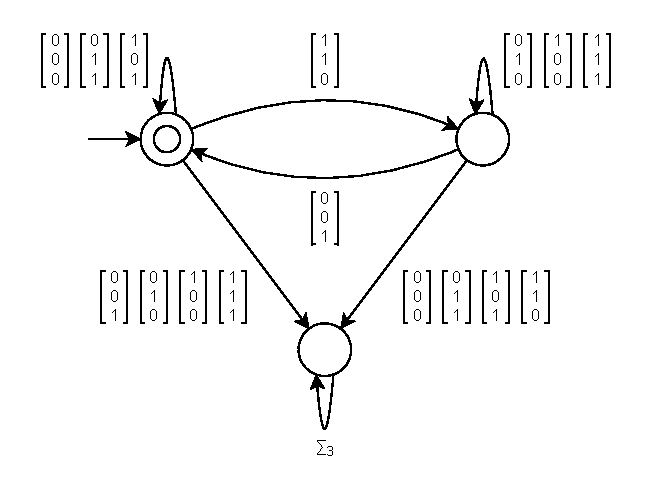
\includegraphics[scale=0.8]{Figures/Problem1.32.pdf} \\
State diagram of a DFA that recognizes $B^{R}$.
\end{center}
\end{proof}

\begin{problem}{1.33}
Let
\[
\Sigma_{2} = 
\left\{
\begin{bmatrix}
    0 \\
    0
\end{bmatrix} ,
\begin{bmatrix}
    0 \\
    1
\end{bmatrix} ,
\begin{bmatrix}
    1 \\
    0
\end{bmatrix} ,
\begin{bmatrix}
    1 \\
    1
\end{bmatrix}
\right\}
\]
\\
Here, $\Sigma_{2}$ contains all columns of 0s and 1s of height two. A string of symbols in $\Sigma_{2}$ gives two rows of 0s and 1s. Consider each row to be a binary number and let
\[
C = 
\left\{
w \, \in \, \Sigma_{2}^{*} \, | \, the \, bottom \, row \, of \, w \, is \, three  \, times \, the \, top \, row
\right\}
\]
For example,
\[
\begin{bmatrix}
    0 \\
    0
\end{bmatrix}
\begin{bmatrix}
    1 \\
    0
\end{bmatrix}
\begin{bmatrix}
    1 \\
    1
\end{bmatrix}
\begin{bmatrix}
    0 \\
    0
\end{bmatrix} \in \, C, \, but
\begin{bmatrix}
    0 \\
    1
\end{bmatrix}
\begin{bmatrix}
    0 \\
    1
\end{bmatrix}
\begin{bmatrix}
    1 \\
    0
\end{bmatrix} \not\in \, C. 
\]
Show that C is regular.
\end{problem}

\begin{idea}
To prove $C$ is regular, we show that $C$'s reverse $C^{R}$ is regular. According to the proof given in Problem 1.31, if $C^{R}$ is regular, then its reverse $C$ is also regular.
\end{idea}

\begin{center}
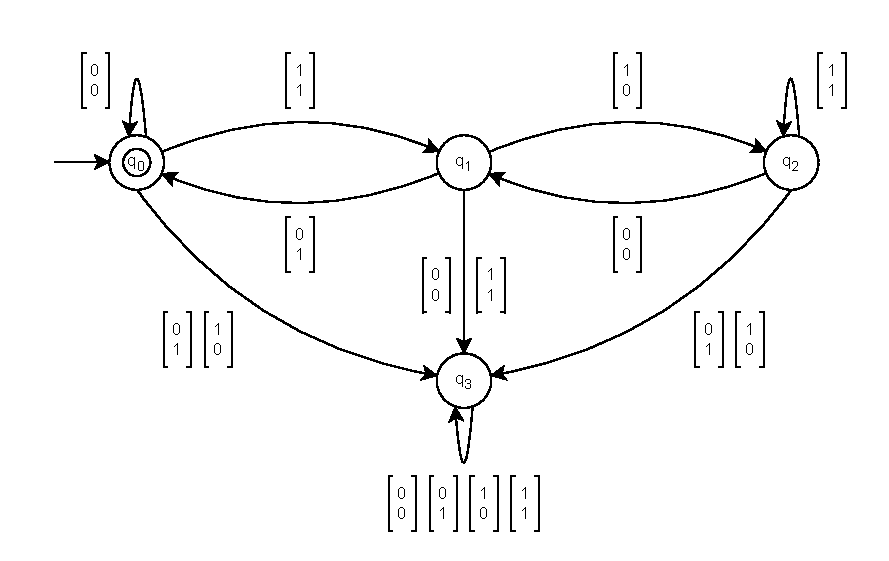
\includegraphics[scale=0.8]{Figures/Problem1.33.pdf} \\
State diagram of a DFA that recognizes $C^{R}$.
\end{center}

\begin{proof}
The proof is by construction. The above state diagram shows the construction of a DFA that recognizes $C^{R}$.
\end{proof}

\begin{problem}{1.34}
Let $\Sigma_{2}$ be the same as in Problem 1.33. Consider each row to be a binary number and let
\[
D = 
\left\{
w \in \Sigma_{2}^{*} \; | \; the \; top \; row \; of \; w \; is \; a \; larger \; number \; than \; is \; the \; bottom \; row
\right\}
\]
For example,
\[
\begin{bmatrix}
    0 \\
    0
\end{bmatrix}
\begin{bmatrix}
    1 \\
    0
\end{bmatrix}
\begin{bmatrix}
    1 \\
    1
\end{bmatrix}
\begin{bmatrix}
    0 \\
    0
\end{bmatrix} \in D, \, but
\begin{bmatrix}
    0 \\
    0
\end{bmatrix}
\begin{bmatrix}
    0 \\
    1
\end{bmatrix}
\begin{bmatrix}
    1 \\
    1
\end{bmatrix}
\begin{bmatrix}
    0 \\
    0
\end{bmatrix} \not\in D
\]
Show that D is regular.
\end{problem}

\begin{center}
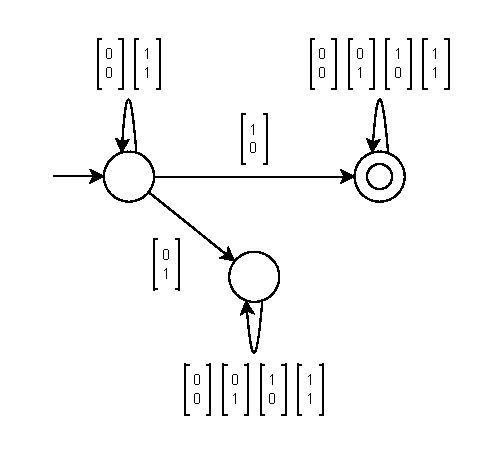
\includegraphics[scale=0.9]{Figures/Problem1.34.pdf} \\
State diagram of a DFA that recognizes $D$.
\end{center}

\begin{proof}
The proof is by construction. The given state diagram shows the construction of a DFA that recognizes $D$.
\end{proof}

\begin{problem}{1.35}
Let $\Sigma_{2}$ be the same as in Problem 1.33. Consider the top and bottom rows to be strings of 0s and 1s, and let
\[
E = 
\left\{
w \in \Sigma_{2}^{*} \; | \; the \; bottom \; row \; of \; w \; is \; the \; reverse \; of \; the \; top \; row
\right\}
\]
Show that $E$ is not regular.
\end{problem}

\begin{proof}
The proof is by contradiction. Assume that $E$ is regular. Let $p$ be the pumping length given by the pumping lemma. Choose $s$ to be the string:
\[
s = 
\left(
\begin{bmatrix}
    1 \\
    0
\end{bmatrix}
\begin{bmatrix}
    1 \\
    0
\end{bmatrix}
\begin{bmatrix}
    1 \\
    0
\end{bmatrix}
\right)^{p}
\left(
\begin{bmatrix}
    0 \\
    1
\end{bmatrix}
\begin{bmatrix}
    0 \\
    1
\end{bmatrix}
\begin{bmatrix}
    0 \\
    1
\end{bmatrix}
\right)^{p}
\]
Therefore, $s \in E$ and $|s| \geq p$, so the pumping lemma guarantees that $s$ can be split into three pieces, $s = xyz$, where for any $i \geq 0$, $xy^{i}z \in E$. According to condition 3 $(i.e. \; |xy| \leq p)$ of the pumping lemma, $y$ can only contain $\begin{bmatrix}1 \\ 0\end{bmatrix}$s. The string $xyyz$ has more $\begin{bmatrix}1 \\ 0\end{bmatrix}$s than $\begin{bmatrix}0 \\ 1\end{bmatrix}$s, so its bottom row is not the reverse of its top row, which is a contradiction. Therefore, $E$ is not regular.
\end{proof}
\end{document}